\documentclass[a4paper,12pt]{article}

\usepackage{amsmath,amssymb,amsthm,multicol,tikz,enumitem}
\usepackage{hyperref}
\usepackage[margin=2cm]{geometry}
\usepackage{fancyvrb}
\usetikzlibrary{calc}

\newcommand\N{\mathbf{N}}
\newcommand\Q{\mathbf{Q}}
\newcommand\R{\mathbf{R}}
\newcommand\Z{\mathbf{Z}}

\newcommand\rem{\textup{rem}}

% Comment out one or the other

\setlength{\parindent}{0pt}

\newcommand\answer[1]{}
\newcommand\ans[1]{}
%\newcommand\notanswer[1]{#1}
%\newcommand\answer[1]{\\[5pt]{\color{blue}{#1}}\hfill{\color{blue}$\qed$}\\[-5pt]}
%\newcommand\ans[1]{{\color{blue}{#1}}}
%\newcommand\notanswer[1]{}



\begin{document}

\begin{center}
{\bf\Huge Midterm 1 Review Topics} \\[5pt]
Data Structures \\
%(4 separate times)\\[5pt]
\textit{*You must justify all your answers to recieve full credit*}
\end{center}

\hrule
\vspace{2pt}
\hrule
\vspace{12pt}

Midterm 1 has 4 theory questions and 1 short C++ program.
Total time is 90 minutes. 

{\small
\begin{enumerate}

\item \textbf{C++ apart from Object Orientation}
\begin{enumerate}[label=1.\Alph*.]
\item Restore/drop parentheses, use syntax trees.
\item Translate between flowcharts and C++ control structures. 
\item Use bit arithmetic.
\item Side-effects in operators, arrays, short-circuit Boolean evaluation.
\item Run pseudocode pointer operations, draw arrows.
\item (C++ code) Perform bit manipulation.
\item (C++ code) Manipulate arrays, char arrays (C-strings), 2D arrays.
\item (C++ code) Input data using "iostream", "sstream", "getLine", "get", "peek"
\end{enumerate}
\item \textbf{C++ with Object Orientation} 
\begin{enumerate}[label=2.\Alph*.]
\item Parameter passing to functions, "const" modifier, default parameters.
\item The order how constructors and destructors are executed.
\item (C++ code) Implement inheritance with virtual/non-virtual functions.
\item (C++ code) Custom comparison function to generic sorting, max or similar algorithm.
\end{enumerate}
\item \textbf{Big-O, Omega, Theta Notation} 
\begin{enumerate}[label=3.\Alph*.]
\item Find the asymptotic growth for a given function.
\item Compare classes of function growth or order them.
\item Express time complexity for recursively defined functions. 
\item Express time complexity for a code snippet ``from the inside out''. 
\item Find the amortized time complexity for an operation on a given data structure.
\item Count the number of calls for comparisons or similar functions.
\end{enumerate}
\item \textbf{Lists, stacks, queues.} 
\begin{enumerate}[label=4.\Alph*.]
\item Use Abstract Data Type (ADT) to write algorithms.
%\item (C++ code) Create an array implementation of some ADT method.
%\item (C++ code) Create a singly linked list implementation of some ADT method.
%\item (C++ code) Create a doubly linked list implementation of some ADT method.
\item (C++ code) Use STL classes for lists, stacks, queues with iterators.
\end{enumerate}
\end{enumerate}
}


\clearpage

\section{C++ apart from Object Orientation}

\begin{enumerate}[label=1.\Alph*.]

\item {\bf Restore/drop parentheses, use syntax trees.}
Use this cheatsheet of operator precedence and associativity, if necessary: \url{https://bit.ly/3Bcigg4}.
\begin{enumerate}
\item Write C++ code that implements the syntax tree shown in the Figure~\ref{fig:abstract-syntax-tree}.
\begin{figure}[!htb]
\center{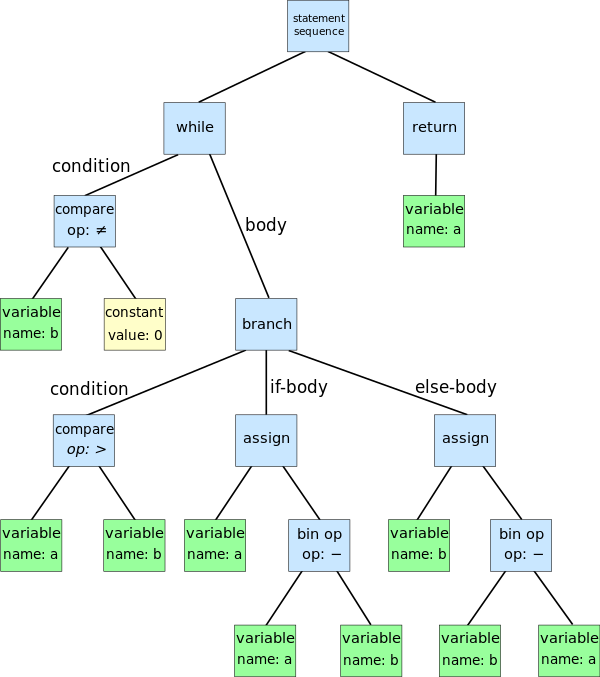
\includegraphics[width=3in]{exam1-review-topics/abstract-syntax-tree.png}}
\caption{\label{fig:abstract-syntax-tree} Syntax Tree}
\end{figure}
\item Draw the abstract syntax tree for this expression: 
\begin{verbatim}
cout << ( a && b + c ? 3 : 5 - d / e ++ / f ) << ( g = h << 17 
== - i > 15) << endl;
\end{verbatim}
In syntax trees leaves are variables such as {\tt cout}, {\tt a}, {\tt b} or numbers. 
Operations such as shifts, Boolean and regular arithmetic are internal nodes.
\item Restore all parentheses in the expression:
\begin{verbatim}
cout << ( a && b + c ? 3 : 5 - d / e ++ / f ) << ( g = h << 17 
== - i > 15) << endl;
\end{verbatim}
\end{enumerate}

\item {\bf Translate between flowcharts and C++ control structures.}
\begin{enumerate}
\item
Draw the flowchart that corresponds to this code snippet: 
\begin{verbatim}
for (int i = 0; i < 3; ++i) {
  switch (a) {
    case 1: if (b > 0) break; 
    case 2: a += 1; 
    case 3: b = a - 17; break;
    default: b = a - 17; continue;
  }
}
\end{verbatim}
Please note that every block in the flowchart belongs to one of the 5 kinds: 
a unique oval-shaped ``Start'' node, a unique oval-shaped ``End'' node, 
rectangular-shaped node with an atomic statement (such as assignment or increment), 
diamond-shaped branch node which checks a condition and has two branches for {\tt true}
and {\tt false}, and finally - a shaded circle-shaped node where two branches 
are joined.
\item Convert the flowchart in Figure~\ref{fig:flowchart} to C++ code: 
\begin{figure}[!htb]
\center{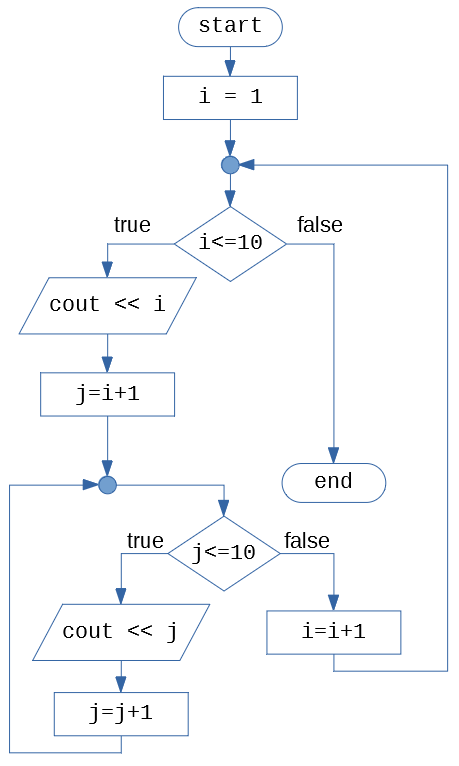
\includegraphics[width=2in]{exam1-review-topics/flowchart.png}}
\caption{\label{fig:flowchart} Syntax Tree}
\end{figure}
\item 
Convert the following code to a flowchart:
\begin{verbatim}
bool a,b;
if (a) 
  if (b) { f(); }
else { g(); }
\end{verbatim}
Is it possible to insert a few curly braces in order to alter the flowchart? 
How can it be done? Write that new version of C++ code.
\end{enumerate}


\item {\bf Use bit arithmetic.} (Bitwise AND, OR, NOT, XOR, left/right shifts.)
\begin{enumerate}
\item Consider the following C++ code fragment computing Bitwise XOR:
\begin{verbatim}
int a = 0x00abcdef;
int x; cin >> x; // 
int b = a^x;
cout << hex << b;
\end{verbatim}
It is known that the expression prints {\tt 01654321}. 
Find the value of {\tt x} that was received from the input.
\item Consider the following C++ code fragment computing Bitwise AND:
\begin{verbatim}
int a = 0x00FF00FF;
int x; cin >> x; // 
int b = a & x;
cout << hex << b;
\end{verbatim}
It is known that the expression prints {\tt 00240068}. 
Find at least two different values of {\tt x} that can give this result.
\item Compute the output of the following code snippet 
without using the computer. (You would need to 
use {\em Two's complement} to get hexadecimal representations
of negative numbers -- \url{https://bit.ly/3EZZ8US}.)
\begin{verbatim}
int a = 17;
int b = -41;
// bitwise AND
cout << hex << (a & b) << endl;
// bitwise OR  
cout << hex << (a | b) << endl;
// bitwise XOR
cout << hex << (a ^ b) << endl;
// bitwise NOT
cout << hex << (~b) << endl;
\end{verbatim}


\end{enumerate}

\item {\bf Side-effects in operators, arrays, short-circuit Boolean evaluation.}
\begin{enumerate}
\item 
\begin{verbatim}
int a[] = {1,3,5,7,9};
int i = 0; 
if ((a[i++] % 2 == 0 && a[i++] - 3) || a[i++] % 3 == 2) { ... }
\end{verbatim}
What is the end-state of the array after the expression in 
{\tt if} statement is evaluated?
\end{enumerate}

\item {\bf Run pseudocode pointer operations, draw arrows.}
\begin{enumerate}
\item We declare the doubly-linked node structure:
\begin{verbatim}
struct Node { int info; Node* prev; Node* next; }
\end{verbatim}
Consider the following structure built from these nodes:
\begin{figure}[!htb]
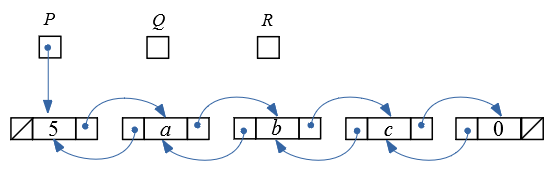
\includegraphics[width=4in]{exam1-review-topics/pointers-and-nodes.png}
\caption{\label{fig:pointers-and-nodes} Pointers and Nodes.}
\end{figure}
Run the following pseudocode and 
draw the nodes and pointer states after Line 7 and Line 12 of the code.
\[ \begin{array}{rl}
1 & Q = P\\
2 & Q = Q\rightarrow next\\
3 & R = Q\rightarrow next\\
4 & \text{\textbf{if\ }} Q\rightarrow info \leq P\rightarrow info\\
5 & \hspace{.5cm} R\rightarrow prev = P\\
6 & \text{\textbf{else\ }}\\
7 & \hspace{.5cm} P\rightarrow  prev = R\\
  & \text{\em (Picture\ 1:\ Show\ the\ pointers\ at\ this\ point) }\\
8 & P\rightarrow next\rightarrow next = R\rightarrow next\\
9 & \text{\textbf{if\ }} R\rightarrow info \leq Q\rightarrow info\\
10 & \hspace{.5cm} R\rightarrow next = P\rightarrow next\\
11 & \text{\textbf{else\ }}\\
12 & \hspace{.5cm} R\rightarrow next = P\rightarrow prev\\
  & \text{\em (Picture\ 2:\ Show\ the\ pointers\ at\ this\ point) }\\
\end{array} \]
\end{enumerate}

\item {\bf (C++ code) Perform bit manipulation.}
\begin{enumerate}
\item Assume that a cryptographer wants to transform every 
{\tt char} into another {\tt char} by applying bit rotation: 
three bits to the right. 
For example, the character {\tt 'C'} with its ASCII code 
{\tt 0x43} (as hex) or {\tt 01000011} (as binary) 
should be transformed into {\tt 01101000}, which is 
hex {\tt 68} or character {\tt 'h'}. 
Complete the function to transform: 
\begin{verbatim}
char transform(char input) {
  // inswert function body to compute bit rotation
  char result = ... 
  return result;
}
\end{verbatim}
\end{enumerate}


\item {\bf (C++ code) Manipulate arrays, char arrays (C-strings), 2D arrays.}
\begin{enumerate}
\item Using {\tt char} pointers only implement function:\\ 
{\tt int myStrcmp(const char * str1, const char * str2 ); }
It should read both strings simultaneously until it reaches terminating character
{\tt \textbackslash{}0} in one of them.\\
It returns $0$, if both strings are identical up to that character.\\
It returns $-1$, if string "str1" is alphabetically before "str2".
(or "str1" is identical with "str2", but terminates sooner).\\
It returns $1$, if string "str1" is alphabetically after "str2".
(or "str1" is identical with "str2", but terminates sooner).

Do not use any predefined string functions, just the "char" pointers
and char comparisons. 
Test this function by the following code:
\begin{verbatim}
// Place the includes, namespaces and your function "myStrcmp" here

int main() {
  cout << myStrcmp("ABC", "ABC"); // prints 0
  cout << myStrcmp("ABC", "ABD"); // prints -1
  cout << myStrcmp("ABC", "ABCD"); // prints -1
  cout << myStrcmp("ABC", "ABB"); // prints 1
  cout << myStrcmp("ABC", "AB"); // prints 1
}
\end{verbatim}


\end{enumerate}


\item {\bf (C++ code) Input data using "iostream", "sstream", "getLine", "get", "peek".}

Write a C++ program that reads standard input from STDIN
(it stops reading when it encounters and empty line -- to linebreaks in a row without any text). 
For each line the program inputs all the integers and adds them. 

{\bf Sample input:}

\begin{verbatim}
1 3 5
1 3 5 7 9 11

4 6
\end{verbatim}

{\bf Sample output:}

\begin{verbatim}
9
36
\end{verbatim}



\end{enumerate}



\section{C++ with Object Orientation}

\begin{enumerate}[label=2.\Alph*.]
\item {\bf Parameter passing to functions, "const" modifier, default parameters.} 
\begin{enumerate} 
\item
The following code shows overloaded method {\tt Square::square} 
with two different parameters -- either one integer or one double. 
What happens, if you call this method on argument {\tt '7'}? 
\begin{verbatim}
#include <iostream> 
using namespace std;
class Square {
  public:
  int square(int a) {  return (a*a); }
  double square(double b) { return b*b; }
};

int main() {
  Square ss;
  cout << ss.square('7') << endl;
}
\end{verbatim}
\item 
What are the values of local variables {\tt a,b} at the 
end of functions {\tt fun()} and {\tt main()} respectively?
\begin{verbatim}
void fun(int a, int& b) {
  a += 10; 
  b += 10;
  // What are the values of a, b here?
}
int main() {
  int a = 13;
  int b = 15; 
  fun(++b,a);
  // What are the values of a, b here?
}
\end{verbatim}
\end{enumerate}

\item {\bf The order how constructors and destructors are executed.}
\begin{enumerate}
\item Consider the following code. 
List the order how the constructors and destructors of 
{\tt Vaccination}, {\tt Employee} and {\tt Manager} 
are invoked. What is the value of {\tt energyPoints} 
of the manager {\tt m2} at the end of this program?

\begin{verbatim}
#include <string>

using namespace std;
class Vaccination {
    public:
    string type {}; 
    int year {}; 
};

class Employee {
    public:
    Vaccination v; 
    int energyPoints; 
    virtual void energize() {
        energyPoints += 100;
    }
};

class Manager: public Employee {
    public:
    Manager(Vaccination v, int energyPoints) {
        this -> v = v;
        this -> energyPoints = energyPoints;
    }
    void energize() {
        energyPoints += 123;
    };
};

void energizeTwice(Employee* e) {
    e -> energize();
    e -> energize();
}

int main() {
    Manager m1 { {"Comirnaty", 2021}, 150};
    Manager m2 = m1; 
    m1.energize();
    energizeTwice(&m2);
    return 0;
}
\end{verbatim}



\end{enumerate}
\item {\bf (C++ code) Implement inheritance with virtual/non-virtual functions.}

\begin{enumerate}
\item What is the {\tt width} and {\tt height} of both the squares
{\tt s1} and {\tt s2} at the end of the program: 

\begin{verbatim}
#include <iostream>
#include <string>

using namespace std;
class Rectangle {
    protected:
    int width, height; 
    public:
    string color;
    Rectangle(int width, int height) {
        this->width = width; 
        this->height = height;
        color = "gray";
    }    

    void makeWider() {
        width *= 2; 
    }
};

class Square: public Rectangle {
    public:
    Square(int size): Rectangle(size, size) {
        color = "red";        
    }
    void makeWider() {
        width *= 2;
        height *= 2;
    }
};

int main() {
    Square s1(17);
    Square s2 = s1;
    s1.makeWider();
    Rectangle* r2 = &s2;
    r2 -> makeWider();
}
\end{verbatim}
\end{enumerate}


\item {\bf (C++ code) Custom comparison function to sorting, max or similar algorithm.}

Finish the implementation of method main: 
It should read in student ages and heights and output the "maximal student" -- 
the student who has the largest age (if there are multiple students of the 
same age, output the tallest one). 

\begin{verbatim}
#include <iostream>
#include <iomanip> 
#include <set>

using namespace std;
struct Student {
  int age;
  double height;
  Student(int aa = 1, double hh = 1): 
          age(aa), height(hh) {}

  friend istream &operator>>(
    istream  &input, Student &S ) { 
      input >> S.age >> S.height;
      return input;            
  }

  friend ostream &operator<<(ostream &output, const Student &S ) { 
      output << "Student(" << S.age << "," << std::fixed << 
          std::setprecision(5) << S.height << ")";
      return output;            
  }

  friend bool operator<(const Student &left, const Student &right) {
      return (left.age<right.age) || 
	  (left.age == right.height && left.height<right.height);
  }
};

int main() {
  // read in 10 students into a STL class "vector" 
  // find the maximum student (the tallest among the eldest ones)
  // output that maximum student to "cout". 
}
\end{verbatim}


\end{enumerate}






\section{Big-O, Omega, Theta Notation}

\begin{enumerate}[label=3.\Alph*.]
\item {\bf Find the asymptotic growth for a given function.}
\begin{enumerate} 
\item Define the following function $f(n)$ 
\[ f(n) = n^{\log_{10} n} + (1 + \sin (n)) n^{10}. \]
Find optimal asymptotic $g_1(n)$ (upper estimate) and $g_2(n)$ (lower extimate).
Namely, we should have 
$f(n)$ is in $O(g_1(n))$ and $f(n)$ is in $\Omega(g_2(n))$.
\end{enumerate}
\item {\bf Compare classes of function growth or order them.}
\begin{enumerate} 
\item Rank the following functions so that for every two functions $g_i(n)$ 
and $g_j(n)$ in this ordering, $g_i(n)$ is to the left of $g_j(n)$ iff
$g_i(n)$ is in $O(g_j(n))$. 
\[ g_1(n) = n^e,\;\; g_2(n) = e^n,\;\; g_3(n) = {n \choose 5},\;\; g_4(n) = \sqrt{2^{\sqrt{n}}}, \]
\[ g_5(n) = {n \choose n-4},\;\; g_6(n) = 2^{5(\log_2 n)^3},\;\; g_7(n) = n^{(\log_2 n)^2},\;\;
g_8(n) = n^3 \cdot {n \choose 3}. 
\]
\end{enumerate}
\item {\bf Express time complexity for recursively defined functions.}
\begin{enumerate} 
\item 
Find some $\Theta(g(n))$ containing the function satisfying the 
following recurrence: 
\[ \left\{ \begin{array}{l}
T(n) = 1, \mbox{if $n \leq 2$} \\
T(n) = T\left( \left\lceil \frac{n}{3} \right\rceil \right) + T\left( \left\lceil \frac{2n}{3} \right\rceil \right) + n. \\
\end{array} \right. \]
This would be the complexity of an algorithm that receives input of length $n$, splits 
into two unequal parts (of sizes $\lceil n/3 \rceil$ and $\lceil 2n/3 \rceil$) and then applies itself recursively 
(and finally spends $n$ time to combine both computations together). 
\item 
Find an asymptotic solution of the following recurrence:
\[ \left\{ \begin{array}{l}
T(n) = 1,\;\;\mbox{if $n =0$ or $n=1$,} \\
T(n) = \log_2 n + T(\sqrt{n}),\;\;\mbox{if $n > 1$.}\\
\end{array} \right. \]


Express your
answer using $\Theta$-notation, and justify your answer.
\end{enumerate}
\item {\bf Express time complexity for a code snippet ``from the inside out''.}
\begin{enumerate} 
\item {\tt a[i][j]} is an $n \times n$ matrix with integer numbers, and 
here is a function to transform that matrix. 
Find the time complexity of this function as $\Theta(g(n))$. 
\begin{verbatim}
void transform (int** a, int n) {
  for (int i = 0; i < n - 1; i ++) {
    for (int j = i+1; j < n; j++) {
      int tmp = a[i][j];
      a[i][j] = a[j][i];
      a[j][i] = tmp;
    }
  }
}
\end{verbatim}
\end{enumerate}
\item {\bf Find the amortized time complexity for an operation on a given data structure.}
\begin{enumerate}
\item
Somebody is incrementing a 10-digit counter from its initial value {\tt 0000000000} 
to the final value {\tt 9999999999}. 
Changing one digit to a new value in that counter takes $1$ unit of energy. 
In general, changing $k$ digits takes $k$ units of energy. 

For example, incrementing from {\tt 0000000013} to {\tt 0000000014} 
takes $1$ unit of energy (only the last digit changes). 
On the other hand, incrementing from {\tt 0999999999} to {\tt 1000000000} 
takes $10$ units of energy (as all the digits change). 

Find the amortized cost per one increment as the counter moves from the state
{\tt 0000000000} 
to the final state {\tt 9999999999}.
\end{enumerate}

\item {\bf Count the number of calls for comparisons or similar functions.}
\begin{enumerate}
\item Consider the following code to find the 2nd smallest element in an array
of objects {\tt arr[n]} of class {\tt X}, where $n > 2$. 

\begin{verbatim}
bool lessThan(X a, X b) { 
    // some comparison function
}

void swap(X& a, X& b) {
    X temp = a;
    a = b;
    b = temp;
}

X getSecondLargest(X* arr, int n) {
    X smallOne = arr[0];
    X smallTwo = arr[1];
    if (lessThan(smallTwo, smallOne))
        swap(smallOne,smallTwo);
    for (int i = 2; i < n; i++) {
        if (lessThan(arr[i], smallTwo)) 
            smallTwo = arr[i];
        if (lessThan(smallTwo, smallOne))
            swap(smallOne,smallTwo);
    }
    return smallTwo;
}
\end{verbatim}

What is the worst-case number of comparisons (calls to {\tt lessThan(a,b)} 
when finding the second smallest element in an array of length $n$. 
(Try to find the exact count of comparisons; or at least estimate their number with Big-O notation.)
Would it be better to use an efficient sorting algorithm (such as {\tt MergeSort})
on the array, and then pick the second smallest element in the sorted list?
\end{enumerate}
\end{enumerate}


\section{Lists, stacks, queues}

\begin{enumerate}[label=4.\Alph*.]
\item {\bf Use Abstract Data Type (ADT) to write algorithms.}
\begin{enumerate}
\item Given two sorted lists, $L_1$ and $L_2$, write a pseudocode to compute $L_1 \cap L_2$ using only 
the basic list ADT operations. The arguments $L_1$ and $L_2$ can be modified or erased in the process. 
\item 
Given list $L_1$ return the size of it. 
\item 
Given list $L_1$ and value $x$, test if value $x$ is contained in the linked list
\item 
Given list $L_1$ and a value $x$, add $x$ to $L_1$, if it is not already contained in the linked list.
\item 
Given list $L_1$ and a value $x$, remove $x$, if it is contained in the linked list.
\end{enumerate}
\item {\bf (C++ code) Use STL classes for lists, stacks, queues with iterators.}
\begin{enumerate}
\item There are two instances of STL list (containing integers). 
Both of them are represented in non-decreasing order. 
Write a function to merge them into a single STL list (so that it contains the same
elements as in both lists -- in common sorted order). 

\begin{verbatim}
// your implementation of "merge(aa,bb)" 

int main() {
  list<int> aa = { 1,4,7,11  }; 
  list<int> bb = {2,3,5, 8, 13 }; 
  list<int> cc =  merge(aa,bb); 
  // cc should be { 1, 2, 3, 4, 5, 7, 8, 11, 13 }
}
\end{verbatim}
\end{enumerate}
\end{enumerate}


\end{document}
